Referring to Figure~\ref{fig:p3p5-non-concentric}:

\begin{conjecture}
Over 3-periodics in the non-concentric, non-axis-aligned pair, there is some fixed point $P_3$ (resp. $P_5$) such that its power with respect to the circumcircle (resp. Euler circle) is invariant. 
\end{conjecture}

\begin{figure}
    \centering
    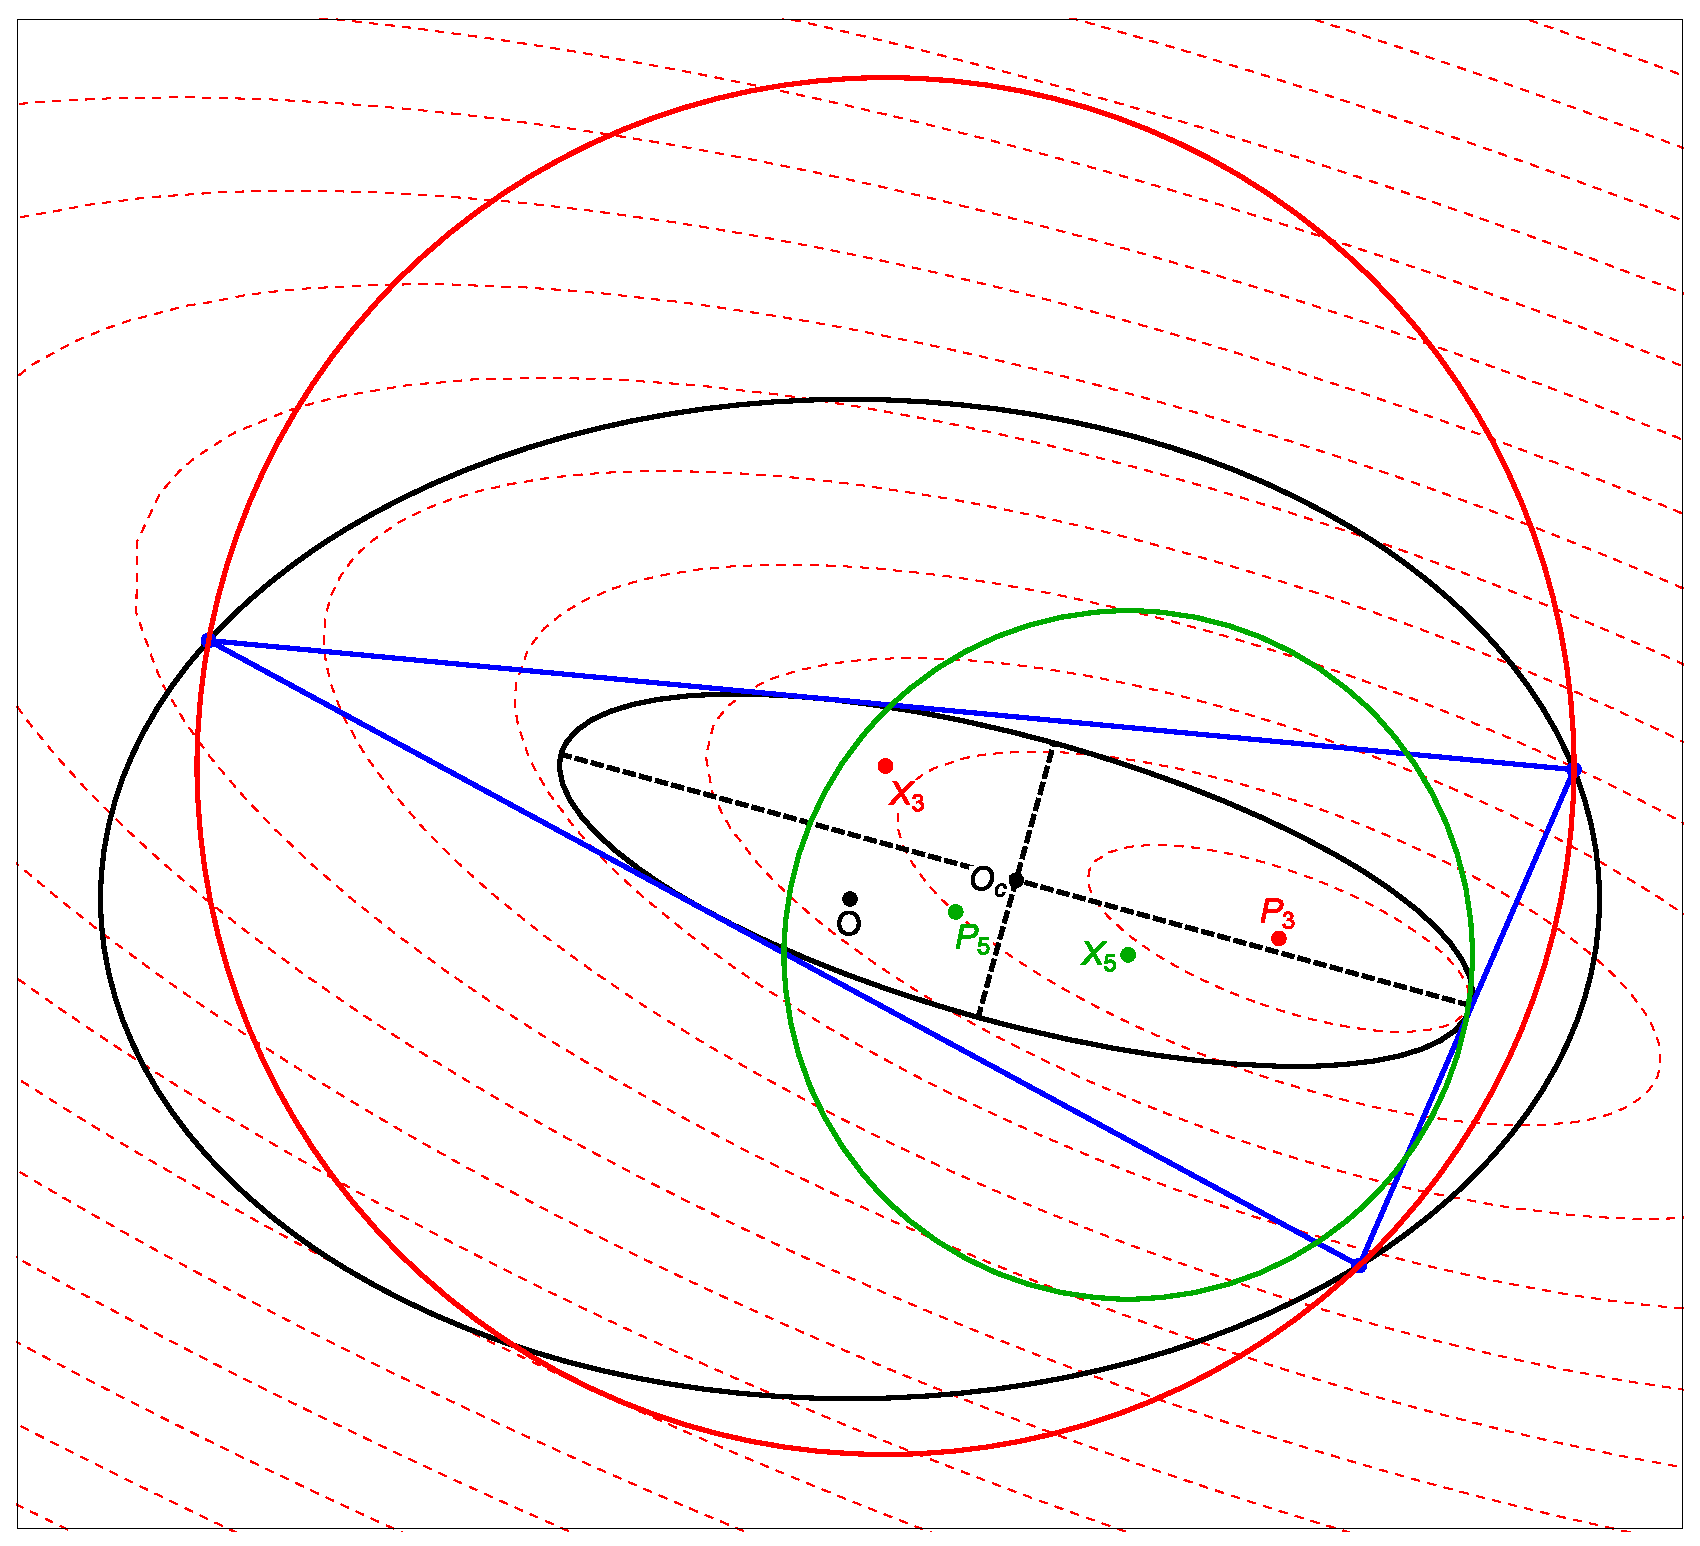
\includegraphics[width=.6\textwidth]{pics/0140_nonconc_tilted_p3p5.eps}
    \caption{Consider a 3-periodics (blue) in a pair of ellipses in general position (centers at $O$ and $O_c$), as well as its circumcircle (red, center $X_3$) and Euler's circle (green, center $X_5$). A point $P_3$ can be numerically located whose power to the circumcircle (solid red) is invariant over the 3-periodic family. Iso-curves of the variance of power of $(x,y)$ with respect to the circumcircle are shown (dashed red): the minimum (and zero) variance occurs at $P_3$. An analogous numeric approach is used to locate the point $P_5$ whose power wrt Euler's circle (solid green) is invariant.}
    \label{fig:p3p5-non-concentric}
\end{figure}

In \cite{olga14,garcia2019-incenter} it is shown that in the confocal pair the locus of the incenter $X_1$ is an ellipse.

Experimentally, we can strengthen Proposition~\ref{prop:concentric}: 

\begin{conjecture}
If the locus of a triangle center $\X$ is an ellipse for all concentric, non-axis-aligned ellipse pairs, then $\X$ is a fixed linear combination of $X_2$ and $X_3$. 
\label{conj:concentric}
\end{conjecture} 

Our very first experimental result was that over 3-periodics in the confocal pair, the locus of the incenter $X_1$ was an ellipse \cite{reznik2011-incenter}. This was subsequently proved \cite{olga14,garcia2019-incenter}. Considering the space of choices of nested ellipse pairs is 5d (5 parameters for each minus 4d homothethy group, minus 1d Cayley condition), little did we know how rare a phenomenon that was (the space of confocal ellipses is a 1d): 

\begin{conjecture}
 The only pair of ellipses admitting Poncelet 3-periodics such that the locus of the incenter $X_1$ is an ellipse is the confocal pair.
\end{conjecture}

\subsection*{Videos} Animations illustrating some phenomena herein are listed on Table~\ref{tab:playlist}.

\begin{table}[H]
\small
\begin{tabular}{|c|l|l|}
\hline
id & Title & \textbf{youtu.be/<.>}\\
\hline
01 & {Cayley-Poncelet Phenomena I: Basics} &
\href{https://youtu.be/virCpDtEvJU}{\texttt{virCpDtEvJU}}\\
02 & {Cayley-Poncelet Phenomena II: Intermediate} &
\href{https://youtu.be/4xsm\_hQU-dE}{\texttt{4xsm\_hQU-dE}}\\
03 & {3-Periodics in Non-Concentric, Unaligned Pair} &
\href{https://youtu.be/bjHpXVyXXVc}{\texttt{bjHpXVyXXVc}}\\
04 & {Loci of Centers I: Generic Pair} &
\href{https://youtu.be/p1medAei_As}{\texttt{p1medAei\_As}}\\
05 & {Loci of Centers II: Pair with Circumcircle} &
\href{https://youtu.be/HXgJQo2UT_8}{\texttt{HXgJQo2UT\_8}}\\
06 & {Loci of Centers III: Concentric Tilted Pair} &
\href{https://youtu.be/hpb7ZgKWjUY}{\texttt{hpb7ZgKWjUY}}\\
07 & {Loci of Centers IV: Outer Ellipse, Inner Non-Concentric Circle} &
\href{https://youtu.be/w7sZ5O8k4xU}{\texttt{w7sZ5O8k4xU}}\\
08 & {3-Periodics in Generic Pair + Affine Image w/ Circumcircle} &
\href{https://youtu.be/6xSFBLWIkTM}{\texttt{6xSFBLWIkTM}}\\
\hline
\end{tabular}
\caption{Videos of some focus-inversive phenomena. The last column is clickable and provides the YouTube code.}
\label{tab:playlist}
\end{table}


